%% knit("nephrops_grid_simulation.Rnw")

\documentclass[12pt]{article}\usepackage[]{graphicx}\usepackage[]{color}
%% maxwidth is the original width if it is less than linewidth
%% otherwise use linewidth (to make sure the graphics do not exceed the margin)
\makeatletter
\def\maxwidth{ %
  \ifdim\Gin@nat@width>\linewidth
    \linewidth
  \else
    \Gin@nat@width
  \fi
}
\makeatother

\definecolor{fgcolor}{rgb}{0.345, 0.345, 0.345}
\newcommand{\hlnum}[1]{\textcolor[rgb]{0.686,0.059,0.569}{#1}}%
\newcommand{\hlstr}[1]{\textcolor[rgb]{0.192,0.494,0.8}{#1}}%
\newcommand{\hlcom}[1]{\textcolor[rgb]{0.678,0.584,0.686}{\textit{#1}}}%
\newcommand{\hlopt}[1]{\textcolor[rgb]{0,0,0}{#1}}%
\newcommand{\hlstd}[1]{\textcolor[rgb]{0.345,0.345,0.345}{#1}}%
\newcommand{\hlkwa}[1]{\textcolor[rgb]{0.161,0.373,0.58}{\textbf{#1}}}%
\newcommand{\hlkwb}[1]{\textcolor[rgb]{0.69,0.353,0.396}{#1}}%
\newcommand{\hlkwc}[1]{\textcolor[rgb]{0.333,0.667,0.333}{#1}}%
\newcommand{\hlkwd}[1]{\textcolor[rgb]{0.737,0.353,0.396}{\textbf{#1}}}%

\usepackage{framed}
\makeatletter
\newenvironment{kframe}{%
 \def\at@end@of@kframe{}%
 \ifinner\ifhmode%
  \def\at@end@of@kframe{\end{minipage}}%
  \begin{minipage}{\columnwidth}%
 \fi\fi%
 \def\FrameCommand##1{\hskip\@totalleftmargin \hskip-\fboxsep
 \colorbox{shadecolor}{##1}\hskip-\fboxsep
     % There is no \\@totalrightmargin, so:
     \hskip-\linewidth \hskip-\@totalleftmargin \hskip\columnwidth}%
 \MakeFramed {\advance\hsize-\width
   \@totalleftmargin\z@ \linewidth\hsize
   \@setminipage}}%
 {\par\unskip\endMakeFramed%
 \at@end@of@kframe}
\makeatother

\definecolor{shadecolor}{rgb}{.97, .97, .97}
\definecolor{messagecolor}{rgb}{0, 0, 0}
\definecolor{warningcolor}{rgb}{1, 0, 1}
\definecolor{errorcolor}{rgb}{1, 0, 0}
\newenvironment{knitrout}{}{} % an empty environment to be redefined in TeX

\usepackage{alltt}
\usepackage{times}
\usepackage{hyperref}
\usepackage{natbib}
\hypersetup{pdfpagemode=UseNone} % don't show bookmarks on initial view
\hypersetup{colorlinks, urlcolor={blue}}

% revise margins
\setlength{\headheight}{0.0in}
\setlength{\topmargin}{0.0in}
\setlength{\headsep}{0.0in}
\setlength{\textheight}{8.65in}
\setlength{\footskip}{0.35in}
\setlength{\oddsidemargin}{0.0in}
\setlength{\evensidemargin}{0.0in}
\setlength{\textwidth}{6.5in}

\setlength{\parskip}{6pt}
\setlength{\parindent}{0pt}

\title{Simulations to assist with \emph{Nephrops} quad-rig trial designs}
\author{For discussion only}
\date{}
\IfFileExists{upquote.sty}{\usepackage{upquote}}{}
\begin{document}



\maketitle

\section{Summary}
A simulation model for abundance-at-length and fishing of \emph{Nephrops} in the Western Irish Sea is developed for the specific purpose of assisting in survey design. The abundance simulation is relatively straightforward, the fishing gear effects are more involved and should only be considered indicative at present. Given time constraints, issues may have arisen with the code so extreme caution is requested in interpreting these results. It is envisaged that the framework will form the basis of further trial designs.  
\section{Simulation setup}
We follow the general model of \citet{Millar:Fryer:1999} to generate catches from three processes:
\begin{enumerate}
 \item Abundance;
 \item Relative fishing intensity;
 \item Contact-selection.
\end{enumerate}

%% TRUE POPULATION
\subsection{Abundance-at-length of \emph{Nephrops}}
The purpose of this section is to simulate a true underlying population of \emph{Nephrops} in terms of abundance-at-length.\\
As the ageing of \emph{Nephrops} is unclear at the moment we assume that there are four components (possibly age classes) present. This can be changed subsequently. First set the population lengths for each component

\begin{knitrout}\footnotesize
\definecolor{shadecolor}{rgb}{0.969, 0.969, 0.969}\color{fgcolor}\begin{kframe}
\begin{alltt}
\hlcom{## median carapace lengths for 4 components}
\hlstd{mu.l} \hlkwb{<-} \hlkwd{c}\hlstd{(}\hlnum{10}\hlstd{,} \hlnum{15}\hlstd{,} \hlnum{20}\hlstd{,} \hlnum{25}\hlstd{)}

\hlcom{## cv of carapace length for each component}
\hlstd{cv.l} \hlkwb{<-} \hlnum{0.3}

\hlcom{## proportion of the population composed of given component}
\hlstd{p} \hlkwb{<-} \hlkwd{c}\hlstd{(}\hlnum{0.4}\hlstd{,} \hlnum{0.3}\hlstd{,} \hlnum{0.2}\hlstd{,} \hlnum{0.1}\hlstd{)}
\end{alltt}
\end{kframe}
\end{knitrout}

Plot the distribution of simulated lengths on the grounds (Figure~\ref{fig:popl}).
\begin{knitrout}\footnotesize
\definecolor{shadecolor}{rgb}{0.969, 0.969, 0.969}\color{fgcolor}\begin{kframe}
\begin{alltt}
\hlcom{## vector of lengths}
\hlstd{length.vec} \hlkwb{<-} \hlnum{0}\hlopt{:}\hlnum{60}

\hlcom{## densities of each component}
\hlstd{d1} \hlkwb{<-} \hlstd{p[}\hlnum{1}\hlstd{]} \hlopt{*} \hlkwd{dlnorm}\hlstd{(length.vec,} \hlkwd{log}\hlstd{(mu.l[}\hlnum{1}\hlstd{]),} \hlkwc{sdlog} \hlstd{= cv.l)}
\hlstd{d2} \hlkwb{<-} \hlstd{p[}\hlnum{2}\hlstd{]} \hlopt{*} \hlkwd{dlnorm}\hlstd{(length.vec,} \hlkwd{log}\hlstd{(mu.l[}\hlnum{2}\hlstd{]),} \hlkwc{sdlog} \hlstd{= cv.l)}
\hlstd{d3} \hlkwb{<-} \hlstd{p[}\hlnum{3}\hlstd{]} \hlopt{*} \hlkwd{dlnorm}\hlstd{(length.vec,} \hlkwd{log}\hlstd{(mu.l[}\hlnum{3}\hlstd{]),} \hlkwc{sdlog} \hlstd{= cv.l)}
\hlstd{d4} \hlkwb{<-} \hlstd{p[}\hlnum{4}\hlstd{]} \hlopt{*} \hlkwd{dlnorm}\hlstd{(length.vec,} \hlkwd{log}\hlstd{(mu.l[}\hlnum{4}\hlstd{]),} \hlkwc{sdlog} \hlstd{= cv.l)}

\hlstd{d} \hlkwb{<-} \hlkwd{rbind}\hlstd{(d1, d2, d3, d4)}

\hlstd{dsum} \hlkwb{<-} \hlkwd{apply}\hlstd{(d,} \hlnum{2}\hlstd{, sum)}

\hlcom{## plot}
\hlkwd{plot}\hlstd{(length.vec, dsum,} \hlkwc{type} \hlstd{=} \hlstr{"n"}\hlstd{,} \hlkwc{xlab} \hlstd{=} \hlstr{"Carapace length (mm)"}\hlstd{,}
     \hlkwc{ylab} \hlstd{=} \hlstr{"Distribution density"}\hlstd{,} \hlkwc{bty} \hlstd{=} \hlstr{"L"}\hlstd{)}

\hlkwd{matlines}\hlstd{(length.vec,} \hlkwd{t}\hlstd{(d),} \hlkwc{col} \hlstd{=} \hlstr{"purple"}\hlstd{,} \hlkwc{lty} \hlstd{=} \hlnum{1}\hlstd{)}

\hlkwd{lines}\hlstd{(length.vec,} \hlkwd{apply}\hlstd{(d,} \hlnum{2}\hlstd{, sum),} \hlkwc{col} \hlstd{=} \hlstr{"forestgreen"}\hlstd{,} \hlkwc{lwd} \hlstd{=} \hlnum{1.5}\hlstd{)}

\hlkwd{legend}\hlstd{(}\hlstr{"topright"}\hlstd{,} \hlkwc{legend} \hlstd{=} \hlkwd{c}\hlstd{(}\hlstr{"Component (age) distribution"}\hlstd{,} \hlstr{"Overall distribution"}\hlstd{),}
       \hlkwc{lty} \hlstd{=} \hlnum{1}\hlstd{,} \hlkwc{lwd} \hlstd{=} \hlkwd{c}\hlstd{(}\hlnum{1}\hlstd{,} \hlnum{1.5}\hlstd{),} \hlkwc{col} \hlstd{=} \hlkwd{c}\hlstd{(}\hlstr{"purple"}\hlstd{,} \hlstr{"forestgreen"}\hlstd{),} \hlkwc{bty} \hlstd{=} \hlstr{"n"}\hlstd{)}
\end{alltt}
\end{kframe}\begin{figure}

{\centering 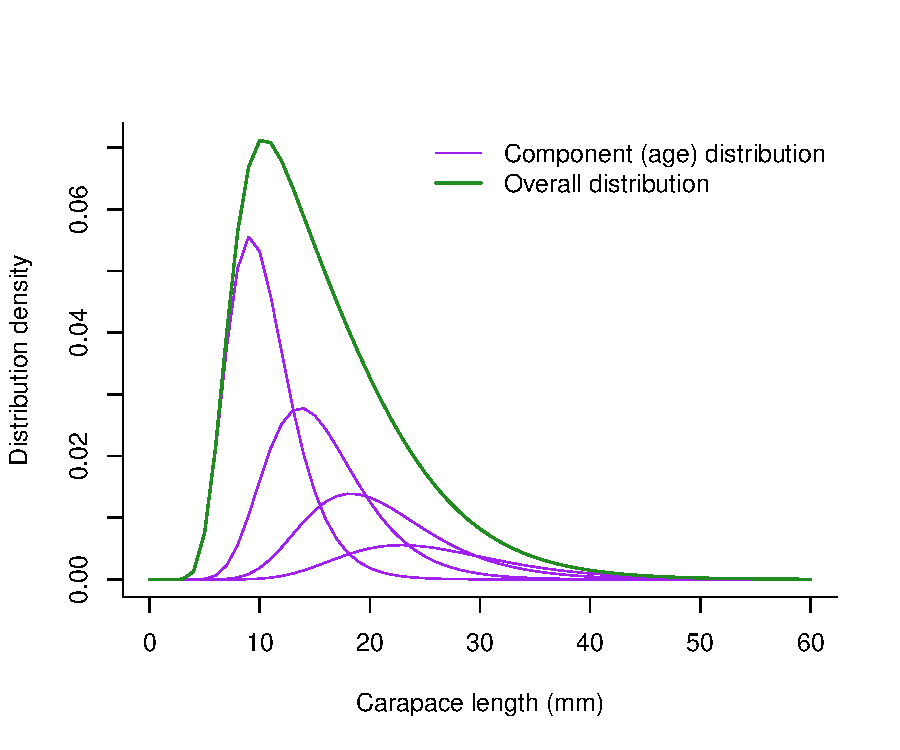
\includegraphics[width=\maxwidth]{figure/popl-1} 

}

\caption[Simulated length distribution of the population of \emph{Nephrops} on the grounds]{Simulated length distribution of the population of \emph{Nephrops} on the grounds.}\label{fig:popl}
\end{figure}


\end{knitrout}
We first assume that the local length distribution (on the grounds) is the same as the population length distribution (Western Irish Sea area). To convert the length distribution to the numbers at length $n_l$ we approximate the overall distribution (Figure~\ref{fig:popl}) by one mm bins, the proportion of the total area occupied by each bin is then used to generate the population counts by length bin. First the proportion of the population per length bin is simulated

\begin{knitrout}\footnotesize
\definecolor{shadecolor}{rgb}{0.969, 0.969, 0.969}\color{fgcolor}\begin{kframe}
\begin{alltt}
\hlcom{## approximate the area under the overall distribution}
\hlkwd{library}\hlstd{(flux)}
\hlstd{midpoints} \hlkwb{<-} \hlstd{(length.vec[}\hlopt{-}\hlkwd{length}\hlstd{(length.vec)]} \hlopt{+} \hlstd{length.vec[}\hlopt{-}\hlnum{1}\hlstd{])}\hlopt{/}\hlnum{2}

\hlstd{nm} \hlkwb{<-} \hlkwd{length}\hlstd{(midpoints)}

\hlcom{## proportion of population per length class}
\hlstd{prop.l} \hlkwb{<-} \hlkwd{rep}\hlstd{(}\hlnum{NA}\hlstd{, nm)}

\hlkwa{for}\hlstd{(i} \hlkwa{in} \hlnum{1}\hlopt{:}\hlstd{(}\hlkwd{length}\hlstd{(length.vec)} \hlopt{-} \hlnum{1}\hlstd{))\{}
  \hlstd{prop.l[i]} \hlkwb{<-} \hlkwd{auc}\hlstd{(}\hlkwc{x} \hlstd{= length.vec[i}\hlopt{:}\hlstd{(i} \hlopt{+} \hlnum{1}\hlstd{)],} \hlkwc{y} \hlstd{= dsum[i}\hlopt{:}\hlstd{(i} \hlopt{+} \hlnum{1}\hlstd{)])}
\hlstd{\}}

\hlkwd{sum}\hlstd{(prop.l)}
\end{alltt}
\begin{verbatim}
## [1] 0.9997978
\end{verbatim}
\begin{alltt}
\hlcom{## close to 1, difference due to approximation}
\end{alltt}
\end{kframe}
\end{knitrout}

The proportion of the population per length bin is then multiplied by the estimated abundance of $4.6 \times 10^9$ burrows \citep{Ligas:etal:survey:2014} to obtain the distribution of numbers at length (Figure~\ref{fig:abundl}).

\begin{knitrout}\footnotesize
\definecolor{shadecolor}{rgb}{0.969, 0.969, 0.969}\color{fgcolor}\begin{kframe}
\begin{alltt}
\hlstd{n} \hlkwb{<-} \hlnum{4.6e9}

\hlstd{nl} \hlkwb{<-} \hlstd{prop.l} \hlopt{*} \hlstd{n}

\hlkwd{barplot}\hlstd{(nl,} \hlkwc{space} \hlstd{=} \hlnum{0}\hlstd{,} \hlkwc{col} \hlstd{=} \hlstr{"lightgrey"}\hlstd{,} \hlkwc{ylab} \hlstd{=} \hlstr{"Abundance (number of burrows)"}\hlstd{,}
        \hlkwc{xlab} \hlstd{=} \hlstr{"Length-class (cm)"}\hlstd{)}

\hlkwd{axis}\hlstd{(}\hlkwc{side} \hlstd{=} \hlnum{1}\hlstd{,} \hlkwc{at} \hlstd{=} \hlkwd{seq}\hlstd{(}\hlnum{0}\hlstd{,} \hlnum{60}\hlstd{,} \hlkwc{by} \hlstd{=} \hlnum{10}\hlstd{))}
\end{alltt}
\end{kframe}\begin{figure}

{\centering 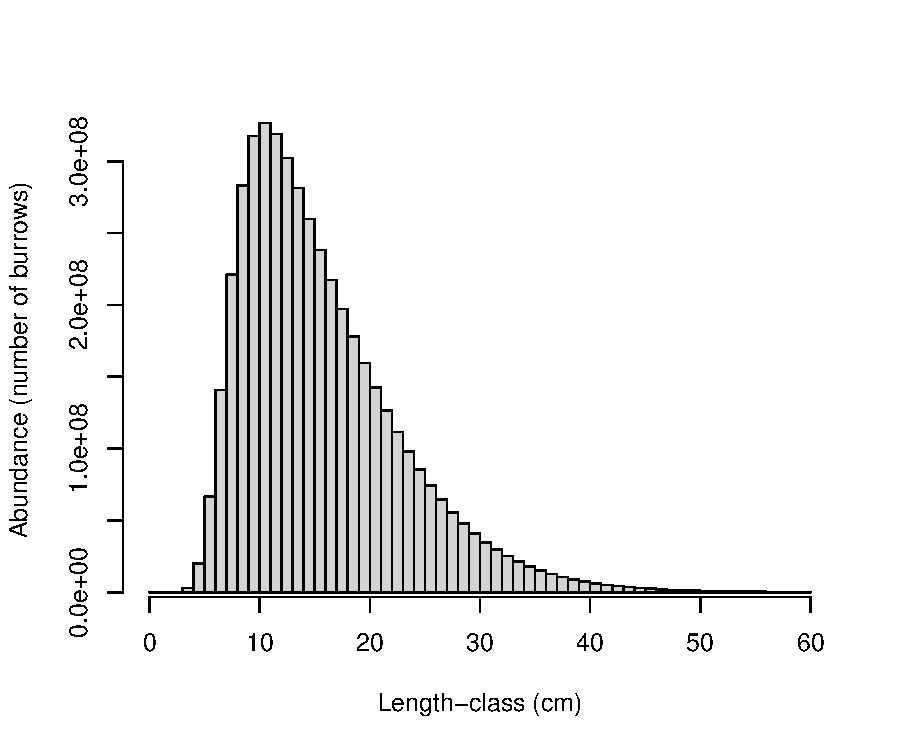
\includegraphics[width=\maxwidth]{figure/abundl-1} 

}

\caption[Simulated abundance-at-length of \emph{Nephrops} on the grounds]{Simulated abundance-at-length of \emph{Nephrops} on the grounds.}\label{fig:abundl}
\end{figure}


\end{knitrout}
It may be necessary to alter the length distribution and abundance spatially to truly reflect the population on the grounds.


\subsection{Contacts with gear}
The footline length on the Celtic Warrior II trials on the Smalls was 38m - assuming the footline takes on a semi-circle during fishing (revise to catenary or similar - think about how this influences the face of each rig also) implies $2 \pi r  = 2 \times 38m$ and so the radius $r  = 38m/\pi$ and the diameter (fishing contact width) is $2 \times 38m/\pi \approx 24.2m$. Based on a towing speed of 3 knots ($\approx$ 5.6km.h$^{-1}$), the area covered per hour is assumed to be 5.6km.h$^{-1}$ $\times$ 0.0242km $\approx$ 0.14km$^2$.h$^{-1}$.

\begin{knitrout}\footnotesize
\definecolor{shadecolor}{rgb}{0.969, 0.969, 0.969}\color{fgcolor}\begin{kframe}
\begin{alltt}
\hlstd{fishing.width} \hlkwb{<-} \hlnum{0.0242} \hlcom{## km}

\hlstd{speed} \hlkwb{<-} \hlnum{5.6} \hlcom{## km/h}

\hlstd{area.ph} \hlkwb{<-} \hlkwd{round}\hlstd{(fishing.width} \hlopt{*} \hlstd{speed,} \hlnum{2}\hlstd{)} \hlcom{## km^2/hour}
\end{alltt}
\end{kframe}
\end{knitrout}

The adjusted mean density is estimated as 0.83 burrows.m$^{-2}$ \citep{Ligas:etal:survey:2014}. Therefore, the simulated number of burrows covered per hour is 0.14km$^2$.h$^{-1}$ $\times$ \ensuremath{8.3\times 10^{5}}km$^{-2}$ $=$ \ensuremath{1.162\times 10^{5}}.h$^{-1}$.\\ 
\begin{knitrout}\footnotesize
\definecolor{shadecolor}{rgb}{0.969, 0.969, 0.969}\color{fgcolor}\begin{kframe}
\begin{alltt}
\hlstd{burrow.dens} \hlkwb{<-} \hlnum{0.83} \hlopt{*} \hlnum{1e6}

\hlstd{(burrows.ph} \hlkwb{<-} \hlstd{area.ph} \hlopt{*} \hlstd{burrow.dens)}
\end{alltt}
\begin{verbatim}
## [1] 116200
\end{verbatim}
\end{kframe}
\end{knitrout}

Assuming a proportion of the \emph{Nephrops} in the burrows covered will come out of the burrows and contact the net (revise), we can simulate the numbers contacting the net per hour. 
\begin{knitrout}\footnotesize
\definecolor{shadecolor}{rgb}{0.969, 0.969, 0.969}\color{fgcolor}\begin{kframe}
\begin{alltt}
\hlstd{contact.prop} \hlkwb{<-} \hlnum{0.2}

\hlstd{hours.towed} \hlkwb{<-} \hlnum{1}

\hlstd{(n.contact} \hlkwb{<-} \hlstd{contact.prop} \hlopt{*} \hlstd{hours.towed} \hlopt{*} \hlstd{burrows.ph)}
\end{alltt}
\begin{verbatim}
## [1] 23240
\end{verbatim}
\end{kframe}
\end{knitrout}

This can then be converted to the numbers at length contacting the net per hour, assuming the probability of contact is equal across length classes.
\begin{knitrout}\footnotesize
\definecolor{shadecolor}{rgb}{0.969, 0.969, 0.969}\color{fgcolor}\begin{kframe}
\begin{alltt}
\hlstd{nl.contact} \hlkwb{<-} \hlstd{n.contact}\hlopt{/}\hlstd{n} \hlopt{*} \hlstd{nl}
\end{alltt}
\end{kframe}
\end{knitrout}

We now have a very basic model \underline{linear} model for generating \emph{Nephrops} contacts with the net on the basis of the numbers of hours towed and density of burrows on the grounds. This could be considerably improved with further discussion and refinement but is assumed correct in the simulations below.

\subsection{Relative fishing intensity}
As in \citep{Millar:Fryer:1999}, the relative fishing intensity $p_j(l)$ is the probability that a fish of length $l$ contacts gear $j$ given that it has contacted the entire net. In a quad-rig, this is the probability that a \emph{Nephrops} entering the entire net contacts each of the rigs. The simplest assumption is that the relative fishing intensity is length-independent and equal across the gears $p_j(l) = 1/4$ (for quad-rig). But it is possible that asymmetries (e.g., door functioning), hydrodynamics, etc. make the probabilities of contact unequal across the nets. We simulate three relative fishing intensity scenarios, assuming length-independence of each:
\begin{enumerate}
  \item Equal relative fishing intensity $p_j(l) = 1/4$;
  \item Single net effect: relative fishing intensity of the second net (second in from port side) fishing twice as well as the others ($p_2(l) = 2/5, p_{1,3,4} = 1/5$).
  \item Simulated door effect: relative fishing intensity increasing from port to starboard with  ($p_1(l) = 1/10, p_2 = 2/10, p_3 = 3/10, p_4 = 4/10$). Note that the relative fishing intensity is drastic with the outermost starboard having four times the fishing intensity of the outermost port. This is unlikely in reality but is used in the simulations to exemplify the effects.
\end{enumerate}

\begin{knitrout}\footnotesize
\definecolor{shadecolor}{rgb}{0.969, 0.969, 0.969}\color{fgcolor}\begin{kframe}
\begin{alltt}
\hlcom{## relative fishing intensity}
\hlcom{## scenario 1}
\hlstd{p.rfi.1} \hlkwb{<-} \hlkwd{rep}\hlstd{(}\hlnum{1}\hlopt{/}\hlnum{4}\hlstd{,} \hlnum{4}\hlstd{)}

\hlcom{## scenario 2}
\hlstd{p.rfi.2} \hlkwb{<-} \hlkwd{c}\hlstd{(}\hlnum{1}\hlopt{/}\hlnum{5}\hlstd{,} \hlnum{2}\hlopt{/}\hlnum{5}\hlstd{,} \hlkwd{rep}\hlstd{(}\hlnum{1}\hlopt{/}\hlnum{5}\hlstd{,} \hlnum{2}\hlstd{))}

\hlcom{## scenario 3}
\hlstd{p.rfi.3} \hlkwb{<-} \hlkwd{c}\hlstd{(}\hlnum{1}\hlopt{/}\hlnum{10}\hlstd{,} \hlnum{2}\hlopt{/}\hlnum{10}\hlstd{,} \hlnum{3}\hlopt{/}\hlnum{10}\hlstd{,} \hlnum{4}\hlopt{/}\hlnum{10}\hlstd{)}
\end{alltt}
\end{kframe}
\end{knitrout}

\subsection{Simulated contact selection $r_j(l)$}
We focus on a much-simplified analysis of the retention of the proportion of \emph{Nephrops} above and below the MLS retained in each cod-end. Given the priority of the cod-end we focus on that here but will add in grid selectivity on (Monday).

\subsubsection{Cod-end retention}
From trials conducted in the Danish fishery over two years, using commercial 90mm diamond mesh codend with 5mm double twine, \citet{Frandsen:etal:2010} estimated $L_{50, 2006} = 16.71, L_{50, 2007} = 18.35$ and $SR_{2006} = 14.71, SR_{2007} = 11.73$. We take an average of these parameters for the selectivity of the 90mm cod-end.

\begin{knitrout}\footnotesize
\definecolor{shadecolor}{rgb}{0.969, 0.969, 0.969}\color{fgcolor}\begin{kframe}
\begin{alltt}
\hlstd{l50.90mm} \hlkwb{<-} \hlstd{(}\hlnum{16.71} \hlopt{+} \hlnum{18.35}\hlstd{)} \hlopt{/} \hlnum{2}

\hlstd{SR.90mm} \hlkwb{<-} \hlstd{(}\hlnum{14.71} \hlopt{+} \hlnum{11.73}\hlstd{)} \hlopt{/} \hlnum{2}
\end{alltt}
\end{kframe}
\end{knitrout}
For the other cod-ends we could not readily find information on the selectivity curves, we therefore assume that each 10mm change in the cod-end mesh size shifts the $L_{50}$ by 5mm, keeping the selectivity range constant (Figure~\ref{fig:codendsel}).

\begin{knitrout}\footnotesize
\definecolor{shadecolor}{rgb}{0.969, 0.969, 0.969}\color{fgcolor}\begin{kframe}
\begin{alltt}
\hlstd{delta} \hlkwb{<-} \hlnum{5} \hlcom{## difference per 10mm}

\hlstd{l50.100mm} \hlkwb{<-} \hlstd{l50.90mm} \hlopt{+} \hlstd{delta}
\hlstd{l50.80mm} \hlkwb{<-} \hlstd{l50.90mm} \hlopt{-} \hlstd{delta}
\hlstd{l50.70mm} \hlkwb{<-} \hlstd{l50.90mm} \hlopt{-} \hlnum{2} \hlopt{*} \hlstd{delta}

\hlcom{## all }
\hlstd{l50} \hlkwb{<-} \hlkwd{c}\hlstd{(l50.70mm, l50.80mm, l50.90mm, l50.100mm)}
\hlkwd{names}\hlstd{(l50)} \hlkwb{<-} \hlkwd{c}\hlstd{(}\hlstr{"70mm"}\hlstd{,} \hlstr{"80mm"}\hlstd{,} \hlstr{"90mm"}\hlstd{,} \hlstr{"100mm"}\hlstd{)}

\hlcom{## selectivity range}
\hlstd{SR.100mm} \hlkwb{<-} \hlstd{SR.80mm} \hlkwb{<-} \hlstd{SR.70mm} \hlkwb{<-} \hlstd{SR.90mm}

\hlcom{## all}
\hlstd{SR} \hlkwb{<-} \hlkwd{c}\hlstd{(SR.70mm, SR.80mm, SR.90mm, SR.100mm)}
\hlkwd{names}\hlstd{(SR)} \hlkwb{<-} \hlkwd{c}\hlstd{(}\hlstr{"70mm"}\hlstd{,} \hlstr{"80mm"}\hlstd{,} \hlstr{"90mm"}\hlstd{,} \hlstr{"100mm"}\hlstd{)}
\end{alltt}
\end{kframe}
\end{knitrout}

\begin{knitrout}\footnotesize
\definecolor{shadecolor}{rgb}{0.969, 0.969, 0.969}\color{fgcolor}\begin{kframe}
\begin{alltt}
\hlstd{logist.sel} \hlkwb{<-} \hlkwa{function}\hlstd{(}\hlkwc{x}\hlstd{,} \hlkwc{l50}\hlstd{,} \hlkwc{sr}\hlstd{)\{}
  \hlkwd{plogis}\hlstd{(}\hlnum{2} \hlopt{*} \hlkwd{log}\hlstd{(}\hlnum{3}\hlstd{)} \hlopt{/} \hlstd{sr} \hlopt{*} \hlstd{(x} \hlopt{-} \hlstd{l50))}
\hlstd{\}}

\hlkwd{curve}\hlstd{(}\hlkwd{logist.sel}\hlstd{(}\hlkwc{x} \hlstd{= x,} \hlkwc{l50} \hlstd{= l50.70mm,} \hlkwc{sr} \hlstd{= SR.70mm),}
      \hlkwc{from} \hlstd{=} \hlnum{0}\hlstd{,} \hlkwc{to} \hlstd{=} \hlnum{60}\hlstd{,} \hlkwc{xlab} \hlstd{=} \hlstr{"Carapace length (mm)"}\hlstd{,}
      \hlkwc{ylab} \hlstd{=} \hlstr{"Proportion retained in cod-end"}\hlstd{,}
      \hlkwc{bty} \hlstd{=} \hlstr{"L"}\hlstd{,} \hlkwc{ylim} \hlstd{=} \hlkwd{c}\hlstd{(}\hlnum{0}\hlstd{,} \hlnum{1}\hlstd{))}
\hlkwd{curve}\hlstd{(}\hlkwd{logist.sel}\hlstd{(}\hlkwc{x} \hlstd{= x,} \hlkwc{l50} \hlstd{= l50.80mm,} \hlkwc{sr} \hlstd{= SR.80mm),}
      \hlkwc{lty} \hlstd{=} \hlnum{2}\hlstd{,} \hlkwc{add} \hlstd{=} \hlnum{TRUE}\hlstd{)}
\hlkwd{curve}\hlstd{(}\hlkwd{logist.sel}\hlstd{(}\hlkwc{x} \hlstd{= x,} \hlkwc{l50} \hlstd{= l50.90mm,} \hlkwc{sr} \hlstd{= SR.90mm),}
      \hlkwc{lty} \hlstd{=} \hlnum{3}\hlstd{,} \hlkwc{add} \hlstd{=} \hlnum{TRUE}\hlstd{)}
\hlkwd{curve}\hlstd{(}\hlkwd{logist.sel}\hlstd{(}\hlkwc{x} \hlstd{= x,} \hlkwc{l50} \hlstd{= l50.100mm,} \hlkwc{sr} \hlstd{= SR.100mm),}
      \hlkwc{lty} \hlstd{=} \hlnum{4}\hlstd{,} \hlkwc{add} \hlstd{=} \hlnum{TRUE}\hlstd{)}
\hlkwd{legend}\hlstd{(}\hlstr{"bottomright"}\hlstd{,} \hlkwc{legend} \hlstd{=} \hlkwd{c}\hlstd{(}\hlstr{"70mm"}\hlstd{,} \hlstr{"80mm"}\hlstd{,} \hlstr{"90mm"}\hlstd{,} \hlstr{"100mm"}\hlstd{),}
       \hlkwc{lty} \hlstd{=} \hlnum{1}\hlopt{:}\hlnum{4}\hlstd{,} \hlkwc{bty} \hlstd{=} \hlstr{"n"}\hlstd{)}
\end{alltt}
\end{kframe}\begin{figure}

{\centering 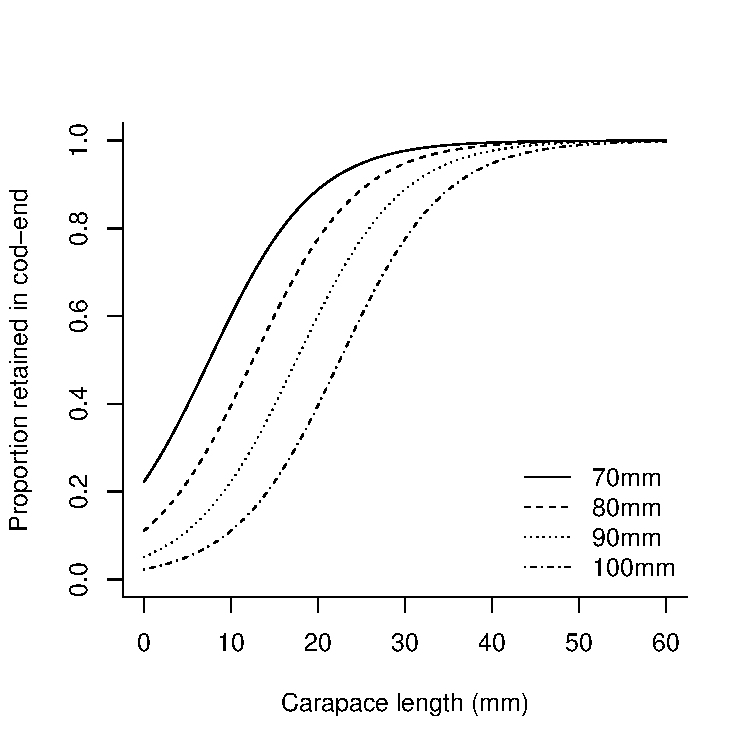
\includegraphics[width=\maxwidth]{figure/codendsel-1} 

}

\caption[Simulated cod-end selectivity curves]{Simulated cod-end selectivity curves. Based on diamond-mesh sizes as indicated in the legend.}\label{fig:codendsel}
\end{figure}

\begin{kframe}\begin{alltt}
\hlcom{## matrix of cod-end retention at length by gear}
\hlstd{rl.mat} \hlkwb{<-} \hlkwd{cbind}\hlstd{(}
            \hlkwd{logist.sel}\hlstd{(}\hlkwc{x} \hlstd{= midpoints,} \hlkwc{l50} \hlstd{= l50.70mm,} \hlkwc{sr} \hlstd{= SR.70mm),}
            \hlkwd{logist.sel}\hlstd{(}\hlkwc{x} \hlstd{= midpoints,} \hlkwc{l50} \hlstd{= l50.80mm,} \hlkwc{sr} \hlstd{= SR.80mm),}
            \hlkwd{logist.sel}\hlstd{(}\hlkwc{x} \hlstd{= midpoints,} \hlkwc{l50} \hlstd{= l50.90mm,} \hlkwc{sr} \hlstd{= SR.90mm),}
            \hlkwd{logist.sel}\hlstd{(}\hlkwc{x} \hlstd{= midpoints,} \hlkwc{l50} \hlstd{= l50.100mm,} \hlkwc{sr} \hlstd{= SR.100mm)}
            \hlstd{)}
\hlkwd{colnames}\hlstd{(rl.mat)} \hlkwb{<-} \hlkwd{c}\hlstd{(}\hlstr{"70mm"}\hlstd{,} \hlstr{"80mm"}\hlstd{,} \hlstr{"90mm"}\hlstd{,} \hlstr{"100mm"}\hlstd{)}
\end{alltt}
\end{kframe}
\end{knitrout}

We do not include weight effects in the simulation here although these could be included by making the parameters of the selectivity curves a function of bulk weight.

\subsection{Net positions}
In a quad-rig with with 4 cod-end mesh sizes, there are 24 possible configurations of the positioning of the nets. To see what configuration gives the maximal difference of mesh sizes between adjacent nets, we can use the permuations.

\begin{knitrout}\footnotesize
\definecolor{shadecolor}{rgb}{0.969, 0.969, 0.969}\color{fgcolor}\begin{kframe}
\begin{alltt}
\hlkwd{library}\hlstd{(combinat)}

\hlstd{perm.list} \hlkwb{<-} \hlkwd{permn}\hlstd{(}\hlkwd{c}\hlstd{(}\hlnum{70}\hlstd{,} \hlnum{80}\hlstd{,} \hlnum{90}\hlstd{,} \hlnum{100}\hlstd{))}

\hlcom{## calulate the differences between the mesh size}
\hlstd{perm.diff} \hlkwb{<-} \hlkwd{unlist}\hlstd{(}\hlkwd{lapply}\hlstd{(perm.list,} \hlkwc{FUN} \hlstd{=} \hlkwa{function}\hlstd{(}\hlkwc{z}\hlstd{)\{}\hlkwd{sum}\hlstd{(}\hlkwd{abs}\hlstd{(}\hlkwd{diff}\hlstd{(z)))\}))}

\hlstd{perm.list[}\hlkwd{which.max}\hlstd{(perm.diff)]} \hlcom{## reverse is also maximal difference}
\end{alltt}
\begin{verbatim}
## [[1]]
## [1]  90  70 100  80
\end{verbatim}
\end{kframe}
\end{knitrout}

We use three net configurations in the simulations:

\begin{enumerate}
  \item Adjacent: 70, 80, 90, 100;
  \item Random: each haul random (completely impractical but useful for comparison);
  %\item Maximal difference: 90, 70, 100, 80.
  \item Non-adjacent: 70, 90, 80, 100.
\end{enumerate}

\begin{knitrout}\footnotesize
\definecolor{shadecolor}{rgb}{0.969, 0.969, 0.969}\color{fgcolor}\begin{kframe}
\begin{alltt}
\hlstd{net.position.adj} \hlkwb{<-} \hlkwd{c}\hlstd{(}\hlstr{"70mm"}\hlstd{,} \hlstr{"80mm"}\hlstd{,} \hlstr{"90mm"}\hlstd{,} \hlstr{"100mm"}\hlstd{)}

\hlstd{net.position.nadj} \hlkwb{<-} \hlkwd{c}\hlstd{(}\hlstr{"70mm"}\hlstd{,} \hlstr{"90mm"}\hlstd{,} \hlstr{"80mm"}\hlstd{,} \hlstr{"100mm"}\hlstd{)}
\end{alltt}
\end{kframe}
\end{knitrout}

\section{Simulation}
The numbers retained in the cod-end per length class $l$ per haul $h$ per gear $j$ are simulated as \citep{Millar:Fryer:1999}:

\begin{equation}
n_{l, j, h} \sim \textnormal{Pois}(p_j \lambda_l r_j(l) e^{\varepsilon_h})
\label{eqn:generalmodel}
\end{equation}
where $\varepsilon_j$ is a haul effect representing unmeasured variables influence on the counts (e.g., some hauls have greater or lower numbers). We assume that this haul effect has a CV of 20\% (refine), corresponding to $\varepsilon_h \sim \textnormal{N}(0, 0.2^2)$. Equation~(\ref{eqn:generalmodel}) gives us the ability to simulate catches per net by haul. We can write a function that produces the expected data per haul

\begin{knitrout}\footnotesize
\definecolor{shadecolor}{rgb}{0.969, 0.969, 0.969}\color{fgcolor}\begin{kframe}
\begin{alltt}
\hlstd{sim.neph.data} \hlkwb{<-} \hlkwa{function}\hlstd{(}\hlkwc{p.rfi}\hlstd{,} \hlkwc{net.position}\hlstd{,} \hlkwc{subs.ratio}\hlstd{,} \hlkwc{CV.haul}\hlstd{,} \hlkwc{hours.towed}\hlstd{)\{}
  \hlcom{##---------------------------  }
  \hlcom{## p.rfi is the relative fishing intensity with names "70mm","80mm","90mm","100mm"}
  \hlcom{## net.position is the order of the nets, e.g., c("70mm","80mm","90mm","100mm")}
  \hlcom{## subs.ratio is the proportion of the catch sampled}
  \hlcom{## CV.haul is the coefficient of variation of the haul effect}
  \hlcom{## hours.towed: number of hourse towed}
  \hlcom{##---------------------------}
  \hlcom{## numbers contacting the net}
  \hlstd{(n.contact} \hlkwb{<-} \hlstd{contact.prop} \hlopt{*} \hlstd{hours.towed} \hlopt{*} \hlstd{burrows.ph)}
  \hlcom{## numbers contacting by length}
  \hlstd{lambda.l} \hlkwb{<-} \hlstd{n.contact}\hlopt{/}\hlstd{n} \hlopt{*} \hlstd{nl}
  \hlcom{## numbers contacting each of the gears}
  \hlstd{nlj} \hlkwb{<-} \hlkwd{matrix}\hlstd{(lambda.l)} \hlopt \hlkwd{t}\hlstd{(}\hlkwd{matrix}\hlstd{(p.rfi))}
  \hlkwd{colnames}\hlstd{(nlj)} \hlkwb{<-} \hlstd{net.position}
  \hlcom{## cod-end retention in order of net position}
  \hlstd{r.l} \hlkwb{<-} \hlstd{rl.mat[, net.position]}
  \hlcom{## haul effect}
  \hlstd{epsilon} \hlkwb{<-} \hlkwd{rnorm}\hlstd{(}\hlnum{1}\hlstd{,} \hlnum{0}\hlstd{, CV.haul)}
  \hlcom{##}
  \hlstd{pois.mean} \hlkwb{<-} \hlstd{nlj} \hlopt{*} \hlstd{r.l} \hlopt{*} \hlkwd{exp}\hlstd{(epsilon)}
  \hlcom{## numbers per net per length class}
  \hlstd{nlh} \hlkwb{<-} \hlkwd{apply}\hlstd{(pois.mean,} \hlnum{2}\hlstd{,} \hlkwc{FUN} \hlstd{=} \hlkwa{function}\hlstd{(}\hlkwc{z}\hlstd{)\{}\hlkwd{rpois}\hlstd{(nm,} \hlkwc{lambda} \hlstd{= z)\})}
  \hlcom{## subsample}
  \hlkwa{for}\hlstd{(i} \hlkwa{in} \hlnum{1}\hlopt{:}\hlnum{4}\hlstd{)\{}
    \hlstd{nlh.all} \hlkwb{<-} \hlkwd{rep}\hlstd{(midpoints,} \hlkwc{times} \hlstd{= nlh[,i])}
    \hlcom{## randomly choose from the total catch }
    \hlstd{n.neph} \hlkwb{<-} \hlkwd{length}\hlstd{(nlh.all)}
    \hlstd{sample.idx} \hlkwb{<-} \hlkwd{sample}\hlstd{(}\hlnum{1}\hlopt{:}\hlstd{n.neph,} \hlkwc{size} \hlstd{=} \hlkwd{round}\hlstd{(n.neph}\hlopt{/}\hlnum{2}\hlstd{),} \hlkwc{replace} \hlstd{=} \hlnum{FALSE}\hlstd{)}
    \hlstd{neph.subsample} \hlkwb{<-} \hlstd{nlh.all[sample.idx]}
    \hlkwd{assign}\hlstd{(}\hlkwd{paste}\hlstd{(}\hlstr{"neph.subsample"}\hlstd{,} \hlkwd{colnames}\hlstd{(nlh)[i],} \hlkwc{sep} \hlstd{=} \hlstr{"."}\hlstd{),}
           \hlstd{neph.subsample)}
    \hlkwd{rm}\hlstd{(neph.subsample)}
  \hlstd{\}}
  \hlcom{##}
  \hlstd{binned.70mm} \hlkwb{<-} \hlkwd{table}\hlstd{(}\hlkwd{cut}\hlstd{(neph.subsample.70mm,} \hlkwc{breaks} \hlstd{= length.vec))}
  \hlstd{binned.80mm} \hlkwb{<-} \hlkwd{table}\hlstd{(}\hlkwd{cut}\hlstd{(neph.subsample.80mm,} \hlkwc{breaks} \hlstd{= length.vec))}
  \hlstd{binned.90mm} \hlkwb{<-} \hlkwd{table}\hlstd{(}\hlkwd{cut}\hlstd{(neph.subsample.90mm,} \hlkwc{breaks} \hlstd{= length.vec))}
  \hlstd{binned.100mm} \hlkwb{<-} \hlkwd{table}\hlstd{(}\hlkwd{cut}\hlstd{(neph.subsample.100mm,} \hlkwc{breaks} \hlstd{= length.vec))}
  \hlcom{##}
  \hlstd{haul.df} \hlkwb{<-} \hlkwd{data.frame}\hlstd{(}\hlkwc{length} \hlstd{= midpoints,}
                        \hlstr{"count.70mm"} \hlstd{=} \hlkwd{as.numeric}\hlstd{(binned.70mm),}
                        \hlstr{"count.80mm"} \hlstd{=} \hlkwd{as.numeric}\hlstd{(binned.80mm),}
                        \hlstr{"count.90mm"} \hlstd{=} \hlkwd{as.numeric}\hlstd{(binned.90mm),}
                        \hlstr{"count.100mm"} \hlstd{=} \hlkwd{as.numeric}\hlstd{(binned.100mm)}
                        \hlstd{)}
  \hlkwd{return}\hlstd{(haul.df)}
\hlstd{\}}
\end{alltt}
\end{kframe}
\end{knitrout}

Test the function (Figure~\ref{fig:exsim}).

\begin{knitrout}\footnotesize
\definecolor{shadecolor}{rgb}{0.969, 0.969, 0.969}\color{fgcolor}\begin{kframe}
\begin{alltt}
\hlstd{sim.haul} \hlkwb{<-} \hlkwd{sim.neph.data}\hlstd{(}\hlkwc{p.rfi} \hlstd{= p.rfi.1,}
                          \hlkwc{net.position} \hlstd{=} \hlkwd{c}\hlstd{(}\hlstr{"70mm"}\hlstd{,} \hlstr{"80mm"}\hlstd{,} \hlstr{"90mm"}\hlstd{,} \hlstr{"100mm"}\hlstd{),}
                          \hlkwc{subs.ratio} \hlstd{=} \hlnum{0.2}\hlstd{,}
                          \hlkwc{CV.haul} \hlstd{=} \hlnum{0.2}\hlstd{,}
                          \hlkwc{hours.towed} \hlstd{=} \hlnum{2}\hlstd{)}

\hlkwd{matplot}\hlstd{(sim.haul[,}\hlnum{1}\hlstd{], sim.haul[,} \hlopt{-}\hlnum{1}\hlstd{],} \hlkwc{pch} \hlstd{=} \hlnum{1}\hlstd{,} \hlkwc{xlab} \hlstd{=} \hlstr{"Carapace length (mm)"}\hlstd{,}
        \hlkwc{ylab} \hlstd{=} \hlstr{"Measured number"}\hlstd{,} \hlkwc{bty} \hlstd{=} \hlstr{"L"}\hlstd{)}
\hlkwd{legend}\hlstd{(}\hlstr{"topright"}\hlstd{,} \hlkwc{legend} \hlstd{=} \hlkwd{c}\hlstd{(}\hlstr{"70mm"}\hlstd{,} \hlstr{"80mm"}\hlstd{,} \hlstr{"90mm"}\hlstd{,} \hlstr{"100mm"}\hlstd{),}
       \hlkwc{pch} \hlstd{=} \hlnum{1}\hlstd{,} \hlkwc{col} \hlstd{=} \hlnum{1}\hlopt{:}\hlnum{4}\hlstd{,} \hlkwc{bty} \hlstd{=} \hlstr{"n"}\hlstd{)}
\end{alltt}
\end{kframe}\begin{figure}

{\centering 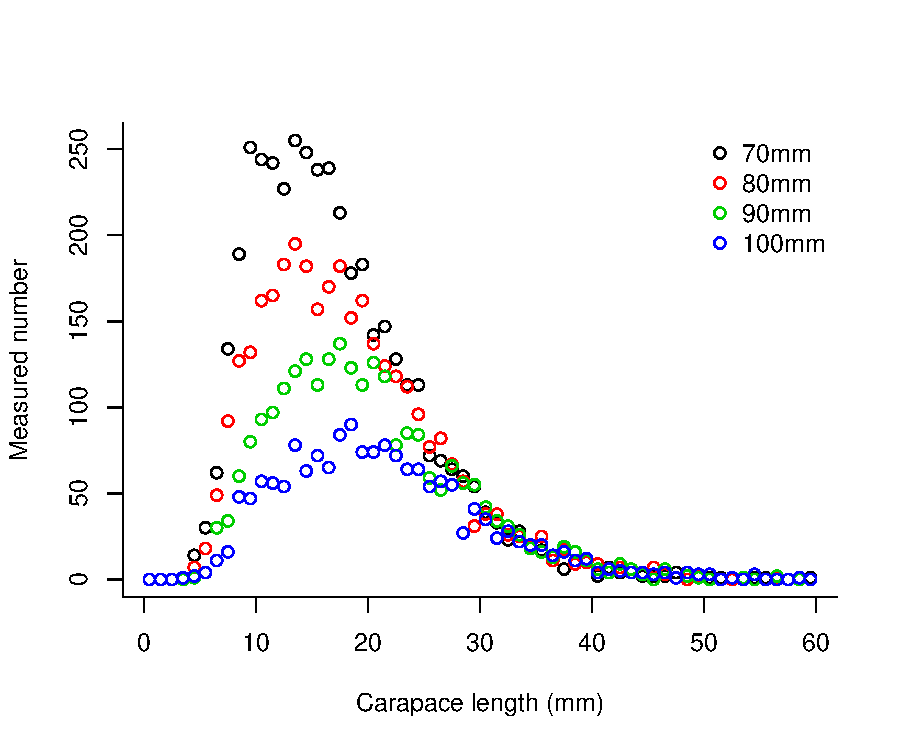
\includegraphics[width=\maxwidth]{figure/exsim-1} 

}

\caption[Simulated sample numbers per length class by mesh size assuming equal fishing intensity]{Simulated sample numbers per length class by mesh size assuming equal fishing intensity.}\label{fig:exsim}
\end{figure}


\end{knitrout}

\subsection{Simulation scenarios}
For the simulation scenarios we define the power as the power to detect a significant ($\alpha = 0.05$) difference in the number caught below the minimum landing size (20mm) by gear with the direction of the estimated counts being $70mm > 80mm > 90mm > 100mm$. \\

Generate the combinations of simulation scenarios

\begin{knitrout}\footnotesize
\definecolor{shadecolor}{rgb}{0.969, 0.969, 0.969}\color{fgcolor}\begin{kframe}
\begin{alltt}
\hlstd{sim.comb} \hlkwb{<-} \hlkwd{expand.grid}\hlstd{(}\hlkwc{p.rfi} \hlstd{=} \hlkwd{c}\hlstd{(}\hlstr{"p.rfi.1"}\hlstd{,}\hlstr{"p.rfi.2"}\hlstd{,}\hlstr{"p.rfi.3"}\hlstd{),}
                        \hlkwc{net.position} \hlstd{=} \hlkwd{c}\hlstd{(}\hlstr{"adjacent"}\hlstd{,}\hlstr{"random"}\hlstd{,}\hlstr{"non-adjacent"}\hlstd{),}
                        \hlkwc{switch} \hlstd{=} \hlkwd{c}\hlstd{(}\hlstr{"no"}\hlstd{,} \hlstr{"yes"}\hlstd{),}
                        \hlkwc{stringsAsFactors} \hlstd{=} \hlnum{FALSE}\hlstd{)}

\hlstd{sim.comb}\hlopt{$}\hlstd{power} \hlkwb{<-} \hlnum{NA}
\end{alltt}
\end{kframe}
\end{knitrout}


Run through the scenarios with 50 simulations per scenario

\begin{knitrout}\footnotesize
\definecolor{shadecolor}{rgb}{0.969, 0.969, 0.969}\color{fgcolor}\begin{kframe}
\begin{alltt}
\hlstd{nsim} \hlkwb{<-} \hlnum{50}

\hlkwa{for}\hlstd{(i} \hlkwa{in} \hlnum{1}\hlopt{:}\hlkwd{dim}\hlstd{(sim.comb)[}\hlnum{1}\hlstd{])\{}
  \hlkwd{print}\hlstd{(i)}
  \hlstd{sim.correct} \hlkwb{<-} \hlkwd{rep}\hlstd{(}\hlnum{NA}\hlstd{, nsim)}
  \hlcom{##}
  \hlkwa{for}\hlstd{(j} \hlkwa{in} \hlnum{1}\hlopt{:}\hlstd{nsim)\{}
    \hlcom{## get the net position}
    \hlkwa{if}\hlstd{(sim.comb}\hlopt{$}\hlstd{net.position[i]} \hlopt{==} \hlstr{"adjacent"}\hlstd{)\{}
      \hlstd{net.position} \hlkwb{<-} \hlstd{net.position.adj}
    \hlstd{\}}
      \hlkwa{if}\hlstd{(sim.comb}\hlopt{$}\hlstd{net.position[i]} \hlopt{==} \hlstr{"non-adjacent"}\hlstd{)\{}
        \hlstd{net.position} \hlkwb{<-} \hlstd{net.position.nadj}
      \hlstd{\}}
    \hlkwa{if}\hlstd{(sim.comb}\hlopt{$}\hlstd{net.position[i]} \hlopt{==} \hlstr{"random"}\hlstd{)\{}
      \hlstd{net.position} \hlkwb{<-} \hlkwd{sample}\hlstd{(}\hlkwd{c}\hlstd{(}\hlstr{"70mm"}\hlstd{,} \hlstr{"80mm"}\hlstd{,} \hlstr{"90mm"}\hlstd{,} \hlstr{"100mm"}\hlstd{),} \hlnum{4}\hlstd{)}
    \hlstd{\}}
    \hlcom{##}
    \hlstd{nhauls} \hlkwb{<-} \hlnum{10}
    \hlstd{haul.list} \hlkwb{<-} \hlkwd{lapply}\hlstd{(}\hlnum{1}\hlopt{:}\hlstd{nhauls,} \hlkwa{function}\hlstd{(}\hlkwc{x}\hlstd{)\{}
      \hlkwa{if}\hlstd{(sim.comb}\hlopt{$}\hlstd{switch[i]} \hlopt{==} \hlstr{"yes"} \hlopt{&} \hlstd{x} \hlopt{>} \hlnum{5}\hlstd{)\{}
        \hlstd{net.position} \hlkwb{<-} \hlkwd{rev}\hlstd{(net.position)} \hlcom{## rotate the nets}
      \hlstd{\}}
      \hlcom{##print(net.position)}
      \hlstd{dat} \hlkwb{<-} \hlkwd{sim.neph.data}\hlstd{(}\hlkwc{p.rfi} \hlstd{=} \hlkwd{get}\hlstd{(sim.comb}\hlopt{$}\hlstd{p.rfi[i]),}
                           \hlkwc{net.position} \hlstd{= net.position,}
                           \hlkwc{subs.ratio} \hlstd{=} \hlnum{0.2}\hlstd{,}
                           \hlkwc{CV.haul} \hlstd{=} \hlnum{0.2}\hlstd{,}
                           \hlkwc{hours.towed} \hlstd{=} \hlnum{2}\hlstd{)}
      \hlstd{dat}\hlopt{$}\hlstd{HAULID} \hlkwb{<-} \hlstd{x}
      \hlkwd{return}\hlstd{(dat)}
    \hlstd{\})}
    \hlstd{haul.data} \hlkwb{<-} \hlkwd{do.call}\hlstd{(rbind, haul.list)}
    \hlcom{## subset for those under MLS}
    \hlstd{mls.data} \hlkwb{<-} \hlstd{haul.data[haul.data}\hlopt{$}\hlstd{length} \hlopt{<} \hlnum{20}\hlstd{, ]}
    \hlcom{## sum the counts}
    \hlstd{sum.mls.data} \hlkwb{<-} \hlkwd{aggregate}\hlstd{(mls.data[,} \hlopt{-}\hlnum{1}\hlstd{],} \hlkwc{by} \hlstd{=} \hlkwd{list}\hlstd{(mls.data}\hlopt{$}\hlstd{HAULID), sum)}
    \hlcom{## CHECK!! WHEN CHANGES}
    \hlstd{sum.mls.data}\hlopt{$}\hlstd{HAULID} \hlkwb{<-} \hlstd{sum.mls.data}\hlopt{$}\hlstd{HAULID}\hlopt{/}\hlnum{20}
    \hlcom{## }
    \hlstd{sum.mls.data.long} \hlkwb{<-} \hlkwd{reshape}\hlstd{(sum.mls.data,} \hlkwc{direction} \hlstd{=} \hlstr{"long"}\hlstd{,}
                                 \hlkwc{drop} \hlstd{=} \hlkwd{c}\hlstd{(}\hlstr{"Group.1"}\hlstd{),} \hlkwc{varying} \hlstd{=} \hlnum{2}\hlopt{:}\hlnum{5}\hlstd{,} \hlkwc{timevar} \hlstd{=} \hlstr{"Mesh"}\hlstd{)}
    \hlcom{## net position}
    \hlstd{sum.mls.data.long}\hlopt{$}\hlstd{net.pos} \hlkwb{<-} \hlkwd{match}\hlstd{(sum.mls.data.long}\hlopt{$}\hlstd{Mesh, net.position)}
    \hlcom{##}
    \hlkwa{if}\hlstd{(sim.comb}\hlopt{$}\hlstd{switch[i]} \hlopt{==} \hlstr{"yes"}\hlstd{)\{}
      \hlstd{sum.mls.data.long}\hlopt{$}\hlstd{net.pos[sum.mls.data.long}\hlopt{$}\hlstd{HAULID} \hlopt{>} \hlnum{5}\hlstd{]} \hlkwb{<-}
        \hlkwd{match}\hlstd{(sum.mls.data.long}\hlopt{$}\hlstd{Mesh[sum.mls.data.long}\hlopt{$}\hlstd{HAULID} \hlopt{>} \hlnum{5}\hlstd{],} \hlkwd{rev}\hlstd{(net.position))}
      \hlcom{##}
      \hlstd{sum.mls.data.long}\hlopt{$}\hlstd{net.pos} \hlkwb{<-} \hlkwd{factor}\hlstd{(}\hlkwd{paste}\hlstd{(}\hlstr{"pos"}\hlstd{, sum.mls.data.long}\hlopt{$}\hlstd{net.pos,}
                                                \hlkwc{sep} \hlstd{=}\hlstr{""}\hlstd{))}
      \hlcom{##}
      \hlcom{## run the GLMER with position effects }
      \hlstd{mls.glmer} \hlkwb{<-} \hlkwd{glmer}\hlstd{(count} \hlopt{~ -}\hlnum{1} \hlopt{+}  \hlstd{Mesh} \hlopt{+} \hlstd{(}\hlnum{1}\hlopt{|}\hlstd{net.pos),}
                         \hlkwc{data} \hlstd{= sum.mls.data.long,} \hlkwc{family} \hlstd{= poisson)}
      \hlcom{## plot(unlist(ranef(mls.glmer)))}
      \hlstd{null.glmer} \hlkwb{<-} \hlkwd{glmer}\hlstd{(count} \hlopt{~} \hlstd{(}\hlnum{1}\hlopt{|}\hlstd{net.pos),} \hlkwc{data} \hlstd{= sum.mls.data.long,}
                          \hlkwc{family} \hlstd{= poisson)}
      \hlcom{## significance}
      \hlstd{(D} \hlkwb{<-} \hlopt{-} \hlnum{2} \hlopt{*} \hlkwd{logLik}\hlstd{(null.glmer)} \hlopt{+} \hlnum{2} \hlopt{*} \hlkwd{logLik}\hlstd{(mls.glmer))}
      \hlstd{sig} \hlkwb{<-} \hlkwd{pchisq}\hlstd{(D,} \hlkwc{lower.tail} \hlstd{=} \hlnum{FALSE}\hlstd{,} \hlkwc{df} \hlstd{=} \hlnum{3}\hlstd{)}
      \hlcom{## coefficient values}
      \hlstd{coef.hat} \hlkwb{<-} \hlkwd{fixef}\hlstd{(mls.glmer)[}\hlkwd{c}\hlstd{(}\hlstr{"Mesh70mm"}\hlstd{,} \hlstr{"Mesh80mm"}\hlstd{,} \hlstr{"Mesh90mm"}\hlstd{,} \hlstr{"Mesh100mm"}\hlstd{)]}
    \hlstd{\}}\hlkwa{else}\hlstd{\{}
      \hlcom{## run the GLM without position effects }
      \hlstd{mls.glm} \hlkwb{<-} \hlkwd{glm}\hlstd{(count} \hlopt{~ -}\hlnum{1} \hlopt{+}  \hlstd{Mesh,} \hlkwc{data} \hlstd{= sum.mls.data.long,} \hlkwc{family} \hlstd{= poisson)}
      \hlcom{##}
      \hlstd{null.glm} \hlkwb{<-} \hlkwd{glm}\hlstd{(count} \hlopt{~} \hlnum{1}\hlstd{,} \hlkwc{data} \hlstd{= sum.mls.data.long,} \hlkwc{family} \hlstd{= poisson)}
      \hlcom{## significance}
      \hlstd{(D} \hlkwb{<-} \hlopt{-} \hlnum{2} \hlopt{*} \hlkwd{logLik}\hlstd{(null.glm)} \hlopt{+} \hlnum{2} \hlopt{*} \hlkwd{logLik}\hlstd{(mls.glm))}
      \hlstd{sig} \hlkwb{<-} \hlkwd{pchisq}\hlstd{(D,} \hlkwc{lower.tail} \hlstd{=} \hlnum{FALSE}\hlstd{,} \hlkwc{df} \hlstd{=} \hlnum{3}\hlstd{)}
      \hlcom{## coefficient values}
      \hlstd{coef.hat} \hlkwb{<-} \hlkwd{coef}\hlstd{(mls.glm)[}\hlkwd{c}\hlstd{(}\hlstr{"Mesh70mm"}\hlstd{,} \hlstr{"Mesh80mm"}\hlstd{,} \hlstr{"Mesh90mm"}\hlstd{,} \hlstr{"Mesh100mm"}\hlstd{)]}
    \hlstd{\}}
    \hlkwa{if}\hlstd{(}\hlkwd{all}\hlstd{(}\hlkwd{diff}\hlstd{(coef.hat)} \hlopt{<} \hlnum{0}\hlstd{)} \hlopt{&} \hlstd{sig} \hlopt{<} \hlnum{0.05}\hlstd{)\{}
      \hlstd{sim.correct[j]} \hlkwb{<-} \hlnum{1}
    \hlstd{\}}\hlkwa{else}\hlstd{\{}
      \hlstd{sim.correct[j]} \hlkwb{<-} \hlnum{0}
    \hlstd{\}}
  \hlstd{\}}
  \hlcom{##}
  \hlstd{sim.comb}\hlopt{$}\hlstd{power[i]} \hlkwb{<-} \hlkwd{sum}\hlstd{(sim.correct)}\hlopt{/}\hlstd{nsim}
\hlstd{\}}

\hlkwd{save}\hlstd{(}\hlkwc{list} \hlstd{=} \hlkwd{c}\hlstd{(}\hlstr{"sim.comb"}\hlstd{),} \hlkwc{file} \hlstd{=} \hlstr{"sim_comb.RData"}\hlstd{)}
\end{alltt}
\end{kframe}
\end{knitrout}

\begin{kframe}
\begin{alltt}
\hlkwd{load}\hlstd{(}\hlstr{"sim_comb.RData"}\hlstd{)}

\hlstd{sim.comb}\hlopt{$}\hlstd{gear.effect} \hlkwb{<-} \hlkwd{ifelse}\hlstd{(sim.comb}\hlopt{$}\hlstd{p.rfi} \hlopt{==} \hlstr{"p.rfi.1"}\hlstd{,}
                                     \hlstr{"Equal fishing intensity"}\hlstd{,}
                                     \hlkwd{ifelse}\hlstd{(sim.comb}\hlopt{$}\hlstd{p.rfi} \hlopt{==} \hlstr{"p.rfi.2"}\hlstd{,}
                                            \hlstr{"Single net effect"}\hlstd{,}
                                            \hlstr{"Door effect"}\hlstd{)}
                                     \hlstd{)}

\hlstd{sim.comb} \hlkwb{<-} \hlstd{sim.comb[}\hlkwd{order}\hlstd{(sim.comb}\hlopt{$}\hlstd{p.rfi, sim.comb}\hlopt{$}\hlstd{net.position), ]}

\hlkwd{library}\hlstd{(xtable)}

\hlstd{sim.comb.xtab} \hlkwb{<-}
  \hlkwd{xtable}\hlstd{(sim.comb[,} \hlkwd{c}\hlstd{(}\hlstr{"net.position"}\hlstd{,} \hlstr{"gear.effect"}\hlstd{,} \hlstr{"switch"}\hlstd{,} \hlstr{"power"}\hlstd{)])}

\hlkwd{print}\hlstd{(sim.comb.xtab,} \hlkwc{include.rownames} \hlstd{=} \hlnum{FALSE}\hlstd{)}
\end{alltt}
\end{kframe}% latex table generated in R 3.2.1 by xtable 1.7-4 package
% Fri Jul 17 19:05:28 2015
\begin{table}[ht]
\centering
\begin{tabular}{lllr}
  \hline
net.position & gear.effect & switch & power \\ 
  \hline
adjacent & Equal fishing intensity & no & 1.00 \\ 
  adjacent & Equal fishing intensity & yes & 1.00 \\ 
  non-adjacent & Equal fishing intensity & no & 1.00 \\ 
  non-adjacent & Equal fishing intensity & yes & 1.00 \\ 
  random & Equal fishing intensity & no & 1.00 \\ 
  random & Equal fishing intensity & yes & 1.00 \\ 
  adjacent & Single net effect & no & 0.00 \\ 
  adjacent & Single net effect & yes & 0.02 \\ 
  non-adjacent & Single net effect & no & 0.00 \\ 
  non-adjacent & Single net effect & yes & 0.04 \\ 
  random & Single net effect & no & 0.24 \\ 
  random & Single net effect & yes & 0.74 \\ 
  adjacent & Door effect & no & 0.00 \\ 
  adjacent & Door effect & yes & 1.00 \\ 
  non-adjacent & Door effect & no & 0.00 \\ 
  non-adjacent & Door effect & yes & 1.00 \\ 
  random & Door effect & no & 0.08 \\ 
  random & Door effect & yes & 1.00 \\ 
   \hline
\end{tabular}
\end{table}

From these results we can see that:

\begin{itemize}
  \item If the fishing intensity is constant across all the nets (all fishing the same), the power to detect meaningful differences in the numbers caught below the MLS is very high;
  \item If there is a door effect such that the fishing intensity/fishing power decreases or increases across the nets, the power to detect differences will be low without a switch; performing a switch and including the net position as a factor in the analysis results in much improved power to detect;
  \item The most difficult scenario to rectify with the current setup is a single net fishing considerably better than others. Switching does improve this in the random net location by haul but for practical switches it is difficult to isolate what is a gear effect and what is a net effect with a single switch (random effects are assumed symmetric). Additional switches would allow the net position to be included as a fixed effect in the analysis (here they've been necessarily included as a random effect), which may alleviate the issue. This has not been tested here.
\end{itemize}

\bibliography{../../../../misc/epif_bibliography}
\bibliographystyle{../../../../misc/cjfas}
\end{document}












\section{Gear selectivity}
We assume that the gear selection is driven by cod-end retention. We use a logistic selection curve though others can be included (e.g., Richards asymmetric curve).

Convert the lengths to weight (using ICES values here - check), assuming an even sex ratio (revise) (Figure~\ref{fig:lw}).

\begin{knitrout}\footnotesize
\definecolor{shadecolor}{rgb}{0.969, 0.969, 0.969}\color{fgcolor}\begin{kframe}
\begin{alltt}
\hlstd{a} \hlkwb{<-} \hlstd{(}\hlnum{0.00032} \hlopt{+} \hlnum{0.000684}\hlstd{)} \hlopt{/} \hlnum{2}
\hlstd{b} \hlkwb{<-} \hlstd{(}\hlnum{3.210} \hlopt{+} \hlnum{2.963}\hlstd{)} \hlopt{/} \hlnum{2}
\hlkwd{curve}\hlstd{(a} \hlopt{*} \hlstd{x}\hlopt{^}\hlstd{b,} \hlkwc{from} \hlstd{=} \hlnum{0}\hlstd{,} \hlkwc{to} \hlstd{=} \hlnum{40}\hlstd{,} \hlkwc{bty} \hlstd{=} \hlstr{"L"}\hlstd{,}
      \hlkwc{xlab} \hlstd{=} \hlstr{"Carapace length (mm) DOUBLE CHECK"}\hlstd{,} \hlkwc{ylab} \hlstd{=} \hlstr{"Weight (g)"}\hlstd{)}
\end{alltt}
\end{kframe}\begin{figure}

{\centering 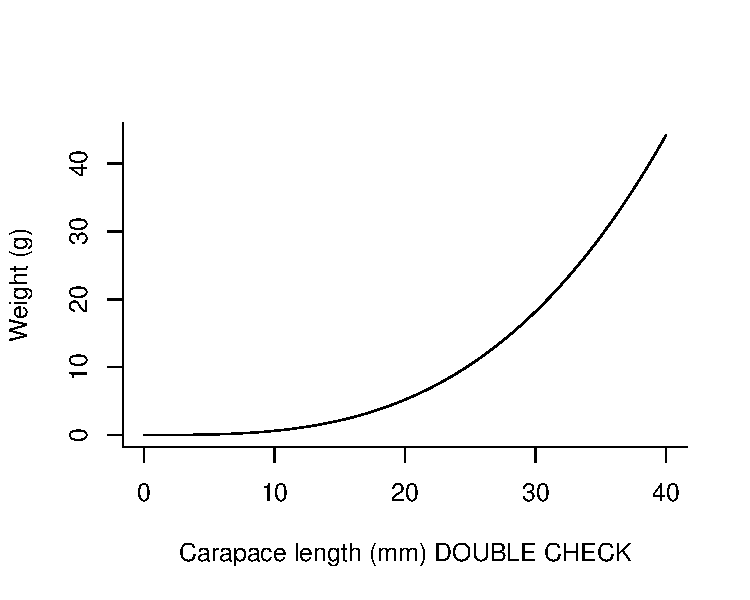
\includegraphics[width=\maxwidth]{figure/lw-1} 

}

\caption[Assumed length-weight relationship for \emph{Nephrops} in the Western Irish Sea]{Assumed length-weight relationship for \emph{Nephrops} in the Western Irish Sea.}\label{fig:lw}
\end{figure}

\begin{kframe}\begin{alltt}
\hlcom{## in kg}
\hlkwd{sum}\hlstd{(nl.contact} \hlopt{*} \hlnum{0.000684} \hlopt{*} \hlstd{midpoints}\hlopt{^}\hlnum{2.963}\hlopt{/}\hlnum{1e3}\hlstd{)}
\end{alltt}
\begin{verbatim}
## [1] 96.17965
\end{verbatim}
\end{kframe}
\end{knitrout}
